%****************************************************************************************************************************************
% File: mpm-ontology.tex
%
% This file is automatically generated. Please do not edit!
%****************************************************************************************************************************************
\section{Ontology Overview}

This ontology captures the Multi-Paradigm Modeling Domain (MPM). It includes concepts for the related modeling, linguistic and formal sub domains.

Figure \ref{fig:mpm_ontology_overview} shows an overview of the MPM ontology. The details of each concept are
provided in the following subsections.

\begin{figure}[!htb]
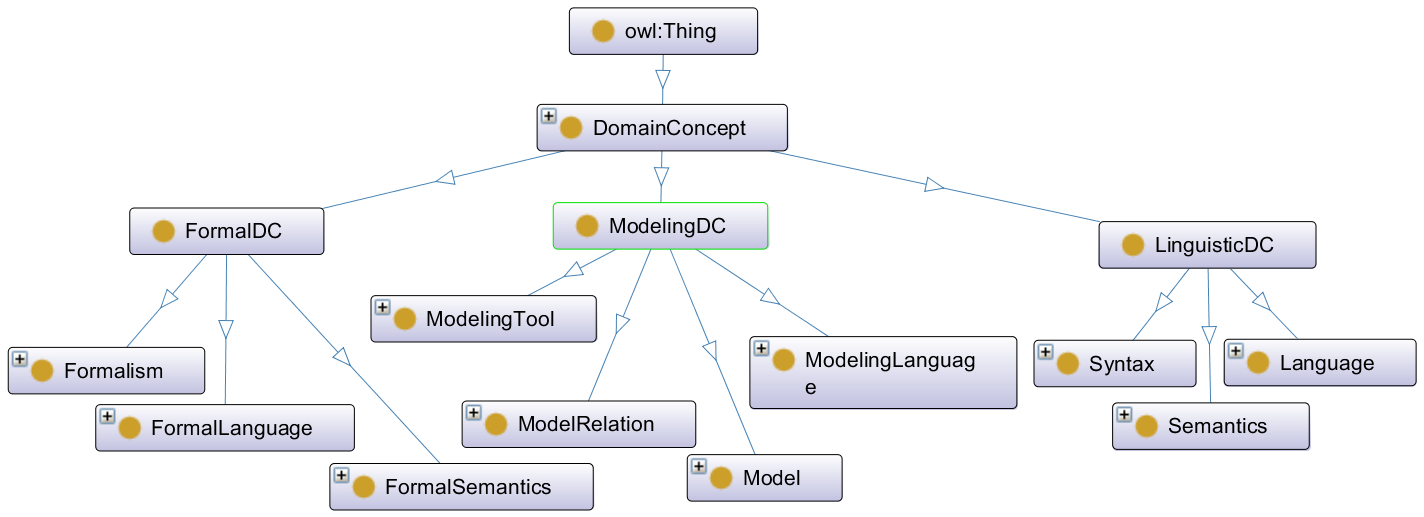
\includegraphics[width=\textwidth]{figures/mpm_ontology_overview.png}
\caption{Overview of the MPM ontology}
\label{fig:mpm_ontology_overview}
\end{figure}



\section{Domain Concepts}

This ontology of multi-paradigm modeling contains concepts divided into sub-domains as presented in the following subsections.

\subsection{FormalDC}
\label{subsecDC:FormalDC}

This class groups domain concepts that are related to the formal aspects of MPM.

\subsubsection{Architecture}
\label{subsubsecC:Architecture}
\didx{Architecture}

https://en.wikipedia.org/wiki/Systems\textunderscore architecture

\textbf{Subclass of}
\begin{itemize}
	\item \textbf{FormalSemantics} (see section \ref{subsubsecC:FormalSemantics})
\end{itemize}






\subsubsection{Behavioral}
\label{subsubsecC:Behavioral}
\didx{Behavioral}

\todoAuthors{Provide ``rdfs:comment'' annotation in ontology}

\textbf{Subclass of}
\begin{itemize}
	\item \textbf{Architecture} (see section \ref{subsubsecC:Architecture})
\end{itemize}






\subsubsection{BehavioralConstraintLanguage}
\label{subsubsecC:BehavioralConstraintLanguage}
\didx{BehavioralConstraintLanguage}

\todoAuthors{Provide ``rdfs:comment'' annotation in ontology}

\textbf{Subclass of}
\begin{itemize}
	\item \textbf{ConstraintLanguage} (see section \ref{subsubsecC:ConstraintLanguage})
\end{itemize}






\subsubsection{Centralized}
\label{subsubsecC:Centralized}
\didx{Centralized}

\todoAuthors{Provide ``rdfs:comment'' annotation in ontology}

\textbf{Subclass of}
\begin{itemize}
	\item \textbf{Deployment} (see section \ref{subsubsecC:Deployment})
\end{itemize}






\subsubsection{Communication}
\label{subsubsecC:Communication}
\didx{Communication}

Communication is the act of conveying intended meanings from one entity or group to another through the use of mutually understood signs and semiotic rules.

\textbf{Subclass of}
\begin{itemize}
	\item \textbf{Behavioral} (see section \ref{subsubsecC:Behavioral})
\end{itemize}






\subsubsection{ConstraintLanguage}
\label{subsubsecC:ConstraintLanguage}
\didx{ConstraintLanguage}

\todoAuthors{Provide ``rdfs:comment'' annotation in ontology}

\textbf{Subclass of}
\begin{itemize}
	\item \textbf{FormalLanguage} (see section \ref{subsubsecC:FormalLanguage})
\end{itemize}






\subsubsection{Deployment}
\label{subsubsecC:Deployment}
\didx{Deployment}

The deployment of a mechanical device, electrical system, computer program, etc., is its assembly or transformation from a packaged form to an operational working state.
Deployment implies moving a product from a temporary or development state to a permanent or desired state.

\textbf{Subclass of}
\begin{itemize}
	\item \textbf{FormalSemantics} (see section \ref{subsubsecC:FormalSemantics})
\end{itemize}






\subsubsection{Distributed}
\label{subsubsecC:Distributed}
\didx{Distributed}

\todoAuthors{Provide ``rdfs:comment'' annotation in ontology}

\textbf{Subclass of}
\begin{itemize}
	\item \textbf{Deployment} (see section \ref{subsubsecC:Deployment})
\end{itemize}






\subsubsection{FormalLanguage}
\label{subsubsecC:FormalLanguage}
\didx{FormalLanguage}

A formal language is a language whose semantics is formally defined. This formal semantics relates to the formalism(s) the language realizes. A formal language has its abstract syntax formally defined.

\textbf{Subclass of}
\begin{itemize}
	\item \textbf{FormalDC} (see section \ref{subsecDC:FormalDC})
	\item \textbf{Language} (see section \ref{subsubsecC:Language})
\end{itemize}






\subsubsection{FormalSemantics}
\label{subsubsecC:FormalSemantics}
\didx{FormalSemantics}

In programming language theory, semantics is the field concerned with the rigorous mathematical study of the meaning of programming languages. It does so by evaluating the meaning of syntactically legal strings defined by a specific programming language, showing the computation involved. In such a case that the evaluation would be of syntactically illegal strings, the result would be non-computation. Semantics describes the processes a computer follows when executing a program in that specific language. This can be shown by describing the relationship between the input and output of a program, or an explanation of how the program will execute on a certain platform, hence creating a model of computation.

\textbf{Subclass of}
\begin{itemize}
	\item \textbf{FormalDC} (see section \ref{subsecDC:FormalDC})
	\item \textbf{Semantics} (see section \ref{subsubsecC:Semantics})
\end{itemize}






\subsubsection{Structural}
\label{subsubsecC:Structural}
\didx{Structural}

Structure is an arrangement and organization of interrelated elements in a material object or system, or the object or system so organized.

\textbf{Subclass of}
\begin{itemize}
	\item \textbf{Architecture} (see section \ref{subsubsecC:Architecture})
\end{itemize}






\subsubsection{StructuralConstraintLanguage}
\label{subsubsecC:StructuralConstraintLanguage}
\didx{StructuralConstraintLanguage}

\todoAuthors{Provide ``rdfs:comment'' annotation in ontology}

\textbf{Subclass of}
\begin{itemize}
	\item \textbf{ConstraintLanguage} (see section \ref{subsubsecC:ConstraintLanguage})
\end{itemize}



\subsection{FormalismDC}
\label{subsecDC:FormalismDC}

This class groups classes related to formalisms

\subsubsection{AutomataBasedFormalism}
\label{subsubsecC:AutomataBasedFormalism}
\didx{AutomataBasedFormalism}

The class of formalisms that are based on automata

\textbf{Subclass of}
\begin{itemize}
	\item \textbf{Formalism} (see section \ref{subsubsecC:Formalism})
\end{itemize}






\subsubsection{BehavioralCharacteristic}
\label{subsubsecC:BehavioralCharacteristic}
\didx{BehavioralCharacteristic}

\todoAuthors{Provide ``rdfs:comment'' annotation in ontology}

\textbf{Subclass of}
\begin{itemize}
	\item \textbf{FormalismCharacteristic} (see section \ref{subsubsecC:FormalismCharacteristic})
\end{itemize}






\subsubsection{ContinuousCharacteristic}
\label{subsubsecC:ContinuousCharacteristic}
\didx{ContinuousCharacteristic}

\todoAuthors{Provide ``rdfs:comment'' annotation in ontology}

\textbf{Subclass of}
\begin{itemize}
	\item \textbf{BehavioralCharacteristic} (see section \ref{subsubsecC:BehavioralCharacteristic})
\end{itemize}






\subsubsection{DiscreteCharacteristic}
\label{subsubsecC:DiscreteCharacteristic}
\didx{DiscreteCharacteristic}

\todoAuthors{Provide ``rdfs:comment'' annotation in ontology}

\textbf{Subclass of}
\begin{itemize}
	\item \textbf{BehavioralCharacteristic} (see section \ref{subsubsecC:BehavioralCharacteristic})
\end{itemize}






\subsubsection{FlowBasedFormalism}
\label{subsubsecC:FlowBasedFormalism}
\didx{FlowBasedFormalism}

\todoAuthors{Provide ``rdfs:comment'' annotation in ontology}

\textbf{Subclass of}
\begin{itemize}
	\item \textbf{Formalism} (see section \ref{subsubsecC:Formalism})
\end{itemize}






\subsubsection{Formalism}
\label{subsubsecC:Formalism}
\didx{Formalism}

Formalisms are mathematical objects consisting of an abstract
syntax and a formal semantics. Languages are concrete
implementations of formalisms. A language has a concrete
syntax, may deviate slightly from the formalism in the
semantics that it implements, or may implement multiple
semantics (e.g., changing the type of numerical solver in a
simulation tool may change the behavior of a model). Also, a
language may implement more than one formalisms.

\textbf{Subclass of}
\begin{itemize}
	\item \textbf{FormalismDC} (see section \ref{subsecDC:FormalismDC})
\end{itemize}


\textbf{References}
\begin{itemize}
	
\item \bibentry{Broman2012}
\end{itemize}




\subsubsection{FormalismCharacteristic}
\label{subsubsecC:FormalismCharacteristic}
\didx{FormalismCharacteristic}

\todoAuthors{Provide ``rdfs:comment'' annotation in ontology}

\textbf{Subclass of}
\begin{itemize}
	\item \textbf{FormalismDC} (see section \ref{subsecDC:FormalismDC})
\end{itemize}






\subsubsection{FormalismFamily}
\label{subsubsecC:FormalismFamily}
\didx{FormalismFamily}

\todoAuthors{Provide ``rdfs:comment'' annotation in ontology}

\textbf{Subclass of}
\begin{itemize}
	\item \textbf{FormalismDC} (see section \ref{subsecDC:FormalismDC})
\end{itemize}






\subsubsection{HybridAutomataBasedFormalism}
\label{subsubsecC:HybridAutomataBasedFormalism}
\didx{HybridAutomataBasedFormalism}

\todoAuthors{Provide ``rdfs:comment'' annotation in ontology}

\textbf{Subclass of}
\begin{itemize}
	\item \textbf{AutomataBasedFormalism} (see section \ref{subsubsecC:AutomataBasedFormalism})
\end{itemize}






\subsubsection{LogicBasedFormalism}
\label{subsubsecC:LogicBasedFormalism}
\didx{LogicBasedFormalism}

\todoAuthors{Provide ``rdfs:comment'' annotation in ontology}

\textbf{Subclass of}
\begin{itemize}
	\item \textbf{Formalism} (see section \ref{subsubsecC:Formalism})
\end{itemize}






\subsubsection{PetriNetBasedFormalism}
\label{subsubsecC:PetriNetBasedFormalism}
\didx{PetriNetBasedFormalism}

Petri nets (also known as a place/transition net or P/T net) are formalisms for the description of distributed systems.

\textbf{Subclass of}
\begin{itemize}
	\item \textbf{Formalism} (see section \ref{subsubsecC:Formalism})
\end{itemize}






\subsubsection{StructureCharacteristic}
\label{subsubsecC:StructureCharacteristic}
\didx{StructureCharacteristic}

\todoAuthors{Provide ``rdfs:comment'' annotation in ontology}

\textbf{Subclass of}
\begin{itemize}
	\item \textbf{FormalismCharacteristic} (see section \ref{subsubsecC:FormalismCharacteristic})
\end{itemize}






\subsubsection{TimedAutomataBasedFormalism}
\label{subsubsecC:TimedAutomataBasedFormalism}
\didx{TimedAutomataBasedFormalism}

\todoAuthors{Provide ``rdfs:comment'' annotation in ontology}

\textbf{Subclass of}
\begin{itemize}
	\item \textbf{HybridAutomataBasedFormalism} (see section \ref{subsubsecC:HybridAutomataBasedFormalism})
\end{itemize}






\subsubsection{TimedCharacteristic}
\label{subsubsecC:TimedCharacteristic}
\didx{TimedCharacteristic}

\todoAuthors{Provide ``rdfs:comment'' annotation in ontology}

\textbf{Subclass of}
\begin{itemize}
	\item \textbf{BehavioralCharacteristic} (see section \ref{subsubsecC:BehavioralCharacteristic})
\end{itemize}






\subsubsection{UncertaintyCharacteristic}
\label{subsubsecC:UncertaintyCharacteristic}
\didx{UncertaintyCharacteristic}

\todoAuthors{Provide ``rdfs:comment'' annotation in ontology}

\textbf{Subclass of}
\begin{itemize}
	\item \textbf{BehavioralCharacteristic} (see section \ref{subsubsecC:BehavioralCharacteristic})
\end{itemize}



\subsection{LinguisticDC}
\label{subsecDC:LinguisticDC}

This class groups domain concepts related to the linguistic aspects of MPM, such as modeling, programming, formal and even natural languages and their syntax.

\subsubsection{AbstractSyntax}
\label{subsubsecC:AbstractSyntax}
\didx{AbstractSyntax}

metamodel

\textbf{Subclass of}
\begin{itemize}
	\item \textbf{Syntax} (see section \ref{subsubsecC:Syntax})
\end{itemize}






\subsubsection{Architecture}
\label{subsubsecC:Architecture}
\didx{Architecture}

https://en.wikipedia.org/wiki/Systems\textunderscore architecture

\textbf{Subclass of}
\begin{itemize}
	\item \textbf{FormalSemantics} (see section \ref{subsubsecC:FormalSemantics})
\end{itemize}






\subsubsection{ArchitectureDescriptionLanguage}
\label{subsubsecC:ArchitectureDescriptionLanguage}
\didx{ArchitectureDescriptionLanguage}

Architecture description languages (ADLs) are used in several disciplines: system engineering, software engineering, and enterprise modelling and engineering.

The system engineering community uses an architecture description language as a language and/or a conceptual model to describe and represent system architectures.

The software engineering community uses an architecture description language as a computer language to create a description of a software architecture. In the case of a so-called technical architecture, the architecture must be communicated to software developers; a functional architecture is communicated to various stakeholders and users. Some ADLs that have been developed are: Acme (developed by CMU), AADL (standardized by the SAE), C2 (developed by UCI), SBC-ADL (developed by National Sun Yat-Sen University), Darwin (developed by Imperial College London), and Wright (developed by CMU).

The up-to-date list of currently existing architectural languages might be found at Up-to-date list of ADLs.

The ISO/IEC/IEEE 42010 document, Systems and software engineering-Architecture description, defines an architecture description language as "any form of expression for use in architecture descriptions" and specifies minimum requirements on ADLs.

The enterprise modeling and engineering community have also developed architecture description languages catered for at the enterprise level. Examples include ArchiMate (now a standard of The Open Group), DEMO, ABACUS (developed by the University of Technology, Sydney). These languages do not necessarily refer to software components, etc. Most of them, however, refer to an application architecture as the architecture that is communicated to the software engineers.

Most of the writing below refers primarily to the perspective from the software engineering community.

\textbf{Subclass of}
\begin{itemize}
	\item \textbf{ModelingLanguage} (see section \ref{subsubsecC:ModelingLanguage})
\end{itemize}






\subsubsection{Behavioral}
\label{subsubsecC:Behavioral}
\didx{Behavioral}

\todoAuthors{Provide ``rdfs:comment'' annotation in ontology}

\textbf{Subclass of}
\begin{itemize}
	\item \textbf{Architecture} (see section \ref{subsubsecC:Architecture})
\end{itemize}






\subsubsection{BehavioralConstraintLanguage}
\label{subsubsecC:BehavioralConstraintLanguage}
\didx{BehavioralConstraintLanguage}

\todoAuthors{Provide ``rdfs:comment'' annotation in ontology}

\textbf{Subclass of}
\begin{itemize}
	\item \textbf{ConstraintLanguage} (see section \ref{subsubsecC:ConstraintLanguage})
\end{itemize}






\subsubsection{Centralized}
\label{subsubsecC:Centralized}
\didx{Centralized}

\todoAuthors{Provide ``rdfs:comment'' annotation in ontology}

\textbf{Subclass of}
\begin{itemize}
	\item \textbf{Deployment} (see section \ref{subsubsecC:Deployment})
\end{itemize}






\subsubsection{Communication}
\label{subsubsecC:Communication}
\didx{Communication}

Communication is the act of conveying intended meanings from one entity or group to another through the use of mutually understood signs and semiotic rules.

\textbf{Subclass of}
\begin{itemize}
	\item \textbf{Behavioral} (see section \ref{subsubsecC:Behavioral})
\end{itemize}






\subsubsection{ConcreteSyntax}
\label{subsubsecC:ConcreteSyntax}
\didx{ConcreteSyntax}

textual/graphics as in AADL

\textbf{Subclass of}
\begin{itemize}
	\item \textbf{Syntax} (see section \ref{subsubsecC:Syntax})
\end{itemize}






\subsubsection{ConstraintLanguage}
\label{subsubsecC:ConstraintLanguage}
\didx{ConstraintLanguage}

\todoAuthors{Provide ``rdfs:comment'' annotation in ontology}

\textbf{Subclass of}
\begin{itemize}
	\item \textbf{FormalLanguage} (see section \ref{subsubsecC:FormalLanguage})
\end{itemize}






\subsubsection{Deployment}
\label{subsubsecC:Deployment}
\didx{Deployment}

The deployment of a mechanical device, electrical system, computer program, etc., is its assembly or transformation from a packaged form to an operational working state.
Deployment implies moving a product from a temporary or development state to a permanent or desired state.

\textbf{Subclass of}
\begin{itemize}
	\item \textbf{FormalSemantics} (see section \ref{subsubsecC:FormalSemantics})
\end{itemize}






\subsubsection{Distributed}
\label{subsubsecC:Distributed}
\didx{Distributed}

\todoAuthors{Provide ``rdfs:comment'' annotation in ontology}

\textbf{Subclass of}
\begin{itemize}
	\item \textbf{Deployment} (see section \ref{subsubsecC:Deployment})
\end{itemize}






\subsubsection{DomainSpecificLanguage}
\label{subsubsecC:DomainSpecificLanguage}
\didx{DomainSpecificLanguage}

A domain-specific language (DSL) is a computer language specialized to a particular application domain. This is in contrast to a general-purpose language (GPL), which is broadly applicable across domains.

\textbf{Subclass of}
\begin{itemize}
	\item \textbf{Language} (see section \ref{subsubsecC:Language})
\end{itemize}






\subsubsection{FormalLanguage}
\label{subsubsecC:FormalLanguage}
\didx{FormalLanguage}

A formal language is a language whose semantics is formally defined. This formal semantics relates to the formalism(s) the language realizes. A formal language has its abstract syntax formally defined.

\textbf{Subclass of}
\begin{itemize}
	\item \textbf{FormalDC} (see section \ref{subsecDC:FormalDC})
	\item \textbf{Language} (see section \ref{subsubsecC:Language})
\end{itemize}






\subsubsection{FormalSemantics}
\label{subsubsecC:FormalSemantics}
\didx{FormalSemantics}

In programming language theory, semantics is the field concerned with the rigorous mathematical study of the meaning of programming languages. It does so by evaluating the meaning of syntactically legal strings defined by a specific programming language, showing the computation involved. In such a case that the evaluation would be of syntactically illegal strings, the result would be non-computation. Semantics describes the processes a computer follows when executing a program in that specific language. This can be shown by describing the relationship between the input and output of a program, or an explanation of how the program will execute on a certain platform, hence creating a model of computation.

\textbf{Subclass of}
\begin{itemize}
	\item \textbf{FormalDC} (see section \ref{subsecDC:FormalDC})
	\item \textbf{Semantics} (see section \ref{subsubsecC:Semantics})
\end{itemize}






\subsubsection{Graphical}
\label{subsubsecC:Graphical}
\didx{Graphical}

\todoAuthors{Provide ``rdfs:comment'' annotation in ontology}

\textbf{Subclass of}
\begin{itemize}
	\item \textbf{ConcreteSyntax} (see section \ref{subsubsecC:ConcreteSyntax})
\end{itemize}






\subsubsection{Language}
\label{subsubsecC:Language}
\didx{Language}

A language is a concrete realization of a set of formalisms. A language has a set of concrete syntaxes. The language may deviate slightly from the formalisms it realizes in the semantics that it realizes, or may realize multiple
semantics.

\textbf{Subclass of}
\begin{itemize}
	\item \textbf{LinguisticDC} (see section \ref{subsecDC:LinguisticDC})
\end{itemize}


\textbf{References}
\begin{itemize}
	
\item \bibentry{Broman2012}
\end{itemize}




\subsubsection{ModelingLanguage}
\label{subsubsecC:ModelingLanguage}
\didx{ModelingLanguage}

A modeling language is any artificial language that can be used to express information or knowledge or systems in a structure that is defined by a consistent set of rules. The rules are used for interpretation of the meaning of components in the structure.

\textbf{Subclass of}
\begin{itemize}
	\item \textbf{Language} (see section \ref{subsubsecC:Language})
	\item \textbf{ModelingDC} (see section \ref{subsecDC:ModelingDC})
\end{itemize}






\subsubsection{ProgrammingLanguages}
\label{subsubsecC:ProgrammingLanguages}
\didx{ProgrammingLanguages}

A programming language is a formal computer language designed to communicate instructions to a machine, particularly a computer. Programming languages can be used to create programs to control the behavior of a machine or to express algorithms.

\textbf{Subclass of}
\begin{itemize}
	\item \textbf{Language} (see section \ref{subsubsecC:Language})
\end{itemize}






\subsubsection{Semantics}
\label{subsubsecC:Semantics}
\didx{Semantics}

Semantics (from Ancient Greek: "significant") is primarily the linguistic, and also philosophical study of meaning in language, programming languages, formal logics, and semiotics. It focuses on the relationship between signifiers-like words, phrases, signs, and symbols-and what they stand for, their denotation.

\textbf{Subclass of}
\begin{itemize}
	\item \textbf{LinguisticDC} (see section \ref{subsecDC:LinguisticDC})
\end{itemize}






\subsubsection{Structural}
\label{subsubsecC:Structural}
\didx{Structural}

Structure is an arrangement and organization of interrelated elements in a material object or system, or the object or system so organized.

\textbf{Subclass of}
\begin{itemize}
	\item \textbf{Architecture} (see section \ref{subsubsecC:Architecture})
\end{itemize}






\subsubsection{StructuralConstraintLanguage}
\label{subsubsecC:StructuralConstraintLanguage}
\didx{StructuralConstraintLanguage}

\todoAuthors{Provide ``rdfs:comment'' annotation in ontology}

\textbf{Subclass of}
\begin{itemize}
	\item \textbf{ConstraintLanguage} (see section \ref{subsubsecC:ConstraintLanguage})
\end{itemize}






\subsubsection{Syntax}
\label{subsubsecC:Syntax}
\didx{Syntax}

\todoAuthors{Provide ``rdfs:comment'' annotation in ontology}

\textbf{Subclass of}
\begin{itemize}
	\item \textbf{LinguisticDC} (see section \ref{subsecDC:LinguisticDC})
\end{itemize}






\subsubsection{Textual}
\label{subsubsecC:Textual}
\didx{Textual}

\todoAuthors{Provide ``rdfs:comment'' annotation in ontology}

\textbf{Subclass of}
\begin{itemize}
	\item \textbf{ConcreteSyntax} (see section \ref{subsubsecC:ConcreteSyntax})
\end{itemize}






\subsubsection{TransformationLanguage}
\label{subsubsecC:TransformationLanguage}
\didx{TransformationLanguage}

A transformation language is a computer language designed to transform some input text in a certain formal language into a modified output text that meets some specific goal.

\textbf{Subclass of}
\begin{itemize}
	\item \textbf{Language} (see section \ref{subsubsecC:Language})
\end{itemize}



\subsection{ModelingDC}
\label{subsecDC:ModelingDC}

This class groups domain concepts related to the modeling aspects of MPM.

\subsubsection{ApplicationMegaModel}
\label{subsubsecC:ApplicationMegaModel}
\didx{ApplicationMegaModel}

A representation of the real models in the CPS development environment.

\textbf{Subclass of}
\begin{itemize}
	\item \textbf{Megamodel} (see section \ref{subsubsecC:Megamodel})
\end{itemize}






\subsubsection{ArchitectureDescriptionLanguage}
\label{subsubsecC:ArchitectureDescriptionLanguage}
\didx{ArchitectureDescriptionLanguage}

Architecture description languages (ADLs) are used in several disciplines: system engineering, software engineering, and enterprise modelling and engineering.

The system engineering community uses an architecture description language as a language and/or a conceptual model to describe and represent system architectures.

The software engineering community uses an architecture description language as a computer language to create a description of a software architecture. In the case of a so-called technical architecture, the architecture must be communicated to software developers; a functional architecture is communicated to various stakeholders and users. Some ADLs that have been developed are: Acme (developed by CMU), AADL (standardized by the SAE), C2 (developed by UCI), SBC-ADL (developed by National Sun Yat-Sen University), Darwin (developed by Imperial College London), and Wright (developed by CMU).

The up-to-date list of currently existing architectural languages might be found at Up-to-date list of ADLs.

The ISO/IEC/IEEE 42010 document, Systems and software engineering-Architecture description, defines an architecture description language as "any form of expression for use in architecture descriptions" and specifies minimum requirements on ADLs.

The enterprise modeling and engineering community have also developed architecture description languages catered for at the enterprise level. Examples include ArchiMate (now a standard of The Open Group), DEMO, ABACUS (developed by the University of Technology, Sydney). These languages do not necessarily refer to software components, etc. Most of them, however, refer to an application architecture as the architecture that is communicated to the software engineers.

Most of the writing below refers primarily to the perspective from the software engineering community.

\textbf{Subclass of}
\begin{itemize}
	\item \textbf{ModelingLanguage} (see section \ref{subsubsecC:ModelingLanguage})
\end{itemize}






\subsubsection{CapturingOperation}
\label{subsubsecC:CapturingOperation}
\didx{CapturingOperation}

The process of capturing information (e.g from users) into a model.

\textbf{Subclass of}
\begin{itemize}
	\item \textbf{TransformationOperation} (see section \ref{subsubsecC:TransformationOperation})
\end{itemize}






\subsubsection{ConfigurationMegaModel}
\label{subsubsecC:ConfigurationMegaModel}
\didx{ConfigurationMegaModel}

Declares types for the models and relations contained in application megamodel. (language and relation types)

\textbf{Subclass of}
\begin{itemize}
	\item \textbf{Megamodel} (see section \ref{subsubsecC:Megamodel})
\end{itemize}






\subsubsection{IntegrationOperation}
\label{subsubsecC:IntegrationOperation}
\didx{IntegrationOperation}

The process to integrate many models together.

\textbf{Subclass of}
\begin{itemize}
	\item \textbf{ModelOperation} (see section \ref{subsubsecC:ModelOperation})
\end{itemize}






\subsubsection{Megamodel}
\label{subsubsecC:Megamodel}
\didx{Megamodel}

A model that contains models and relations between them.

\textbf{Subclass of}
\begin{itemize}
	\item \textbf{Model} (see section \ref{subsubsecC:Model})
\end{itemize}






\subsubsection{MegamodelFragment}
\label{subsubsecC:MegamodelFragment}
\didx{MegamodelFragment}

The fragment is not a complete megamodel, and can't be used alone. It can be reused to take part in another megamodel. (e.g. physical part, view of the system, self-adaptation .... etc.)

\textbf{Subclass of}
\begin{itemize}
	\item \textbf{Model} (see section \ref{subsubsecC:Model})
\end{itemize}





\todoAuthors{Do we add also application and configuration division here?}


\subsubsection{Model}
\label{subsubsecC:Model}
\didx{Model}

A representation of real artifacts regardless of the metamodeling technical space. e.g. xml file, equations...etc.

\textbf{Subclass of}
\begin{itemize}
	\item \textbf{ModelingDC} (see section \ref{subsecDC:ModelingDC})
\end{itemize}






\subsubsection{ModelConstraint}
\label{subsubsecC:ModelConstraint}
\didx{ModelConstraint}

A restriction over model that is input or output for relation

\textbf{Subclass of}
\begin{itemize}
	\item \textbf{ModelingDC} (see section \ref{subsecDC:ModelingDC})
	\item \textbf{Constraint} (see section \ref{subsubsecC:Constraint})
\end{itemize}






\subsubsection{ModelOperation}
\label{subsubsecC:ModelOperation}
\didx{ModelOperation}

It is any kind of transformation from input set of models to output set of models.

\textbf{Subclass of}
\begin{itemize}
	\item \textbf{ModelRelation} (see section \ref{subsubsecC:ModelRelation})
	\item \textbf{Action} (see section \ref{subsubsecC:Action})
\end{itemize}






\subsubsection{ModelRelation}
\label{subsubsecC:ModelRelation}
\didx{ModelRelation}

A relation that connects models.

\textbf{Subclass of}
\begin{itemize}
	\item \textbf{ModelingDC} (see section \ref{subsecDC:ModelingDC})
	\item \textbf{Relation} (see section \ref{subsubsecC:Relation})
\end{itemize}






\subsubsection{ModelingActivity}
\label{subsubsecC:ModelingActivity}
\didx{ModelingActivity}

\todoAuthors{Provide ``rdfs:comment'' annotation in ontology}

\textbf{Subclass of}
\begin{itemize}
	\item \textbf{ModelingDC} (see section \ref{subsecDC:ModelingDC})
	\item \textbf{Activity} (see section \ref{subsubsecC:Activity})
\end{itemize}






\subsubsection{ModelingLanguage}
\label{subsubsecC:ModelingLanguage}
\didx{ModelingLanguage}

A modeling language is any artificial language that can be used to express information or knowledge or systems in a structure that is defined by a consistent set of rules. The rules are used for interpretation of the meaning of components in the structure.

\textbf{Subclass of}
\begin{itemize}
	\item \textbf{Language} (see section \ref{subsubsecC:Language})
	\item \textbf{ModelingDC} (see section \ref{subsecDC:ModelingDC})
\end{itemize}






\subsubsection{ModelingParadigm}
\label{subsubsecC:ModelingParadigm}
\didx{ModelingParadigm}

\todoAuthors{Provide ``rdfs:comment'' annotation in ontology}

\textbf{Subclass of}
\begin{itemize}
	\item \textbf{ModelingDC} (see section \ref{subsecDC:ModelingDC})
\end{itemize}






\subsubsection{ModelingTool}
\label{subsubsecC:ModelingTool}
\didx{ModelingTool}

Tools to model the system.

\textbf{Subclass of}
\begin{itemize}
	\item \textbf{ModelingDC} (see section \ref{subsecDC:ModelingDC})
	\item \textbf{Tool} (see section \ref{subsubsecC:Tool})
\end{itemize}






\subsubsection{TracabilityRelation}
\label{subsubsecC:TracabilityRelation}
\didx{TracabilityRelation}

\todoAuthors{Provide ``rdfs:comment'' annotation in ontology}

\textbf{Subclass of}
\begin{itemize}
	\item \textbf{ModelOperation} (see section \ref{subsubsecC:ModelOperation})
\end{itemize}






\subsubsection{TransformationOperation}
\label{subsubsecC:TransformationOperation}
\didx{TransformationOperation}

The process to transform one model to another.

\textbf{Subclass of}
\begin{itemize}
	\item \textbf{ModelOperation} (see section \ref{subsubsecC:ModelOperation})
\end{itemize}

\section{Properties}


\subsection{hasCharacteristic}
\label{subsecP:hasCharacteristic}
\todoAuthors{Provide ``rdfs:comment'' annotation in ontology}
Subproperty of:
None


Domains:
\begin{itemize}
	\item \textbf{Formalism} (see section \ref{subsubsecC:Formalism})
\end{itemize}


Ranges:
\begin{itemize}
	\item \textbf{FormalismCharacteristic} (see section \ref{subsubsecC:FormalismCharacteristic})
\end{itemize}




\subsection{hasChildFormalism}
\label{subsecP:hasChildFormalism}
\todoAuthors{Provide ``rdfs:comment'' annotation in ontology}
Subproperty of:
None


Domains:
\begin{itemize}
	\item \textbf{FormalismFamily} (see section \ref{subsubsecC:FormalismFamily})
\end{itemize}


Ranges:
\begin{itemize}
	\item \textbf{Formalism} (see section \ref{subsubsecC:Formalism})
\end{itemize}




\subsection{hasChildLanguage}
\label{subsecP:hasChildLanguage}
\todoAuthors{Provide ``rdfs:comment'' annotation in ontology}
Subproperty of:
None


Domains:
\begin{itemize}
	\item \textbf{Language} (see section \ref{subsubsecC:Language})
\end{itemize}


Ranges:
\begin{itemize}
	\item \textbf{Language} (see section \ref{subsubsecC:Language})
\end{itemize}




\subsection{hasContext}
\label{subsecP:hasContext}
\todoAuthors{Provide ``rdfs:comment'' annotation in ontology}
Subproperty of:
None


Domains:
\begin{itemize}
	\item \textbf{ModelOperation} (see section \ref{subsubsecC:ModelOperation})
\end{itemize}


Ranges:
\begin{itemize}
	\item \textbf{ModelOperation} (see section \ref{subsubsecC:ModelOperation})
\end{itemize}




\subsection{hasInput}
\label{subsecP:hasInput}
The model need inputs to do perform the determined task.
Subproperty of:
\begin{itemize}
	\item \textbf{isConnecting} (see section \ref{subsecP:isConnecting})
\end{itemize}


Domains:
\begin{itemize}
	\item \textbf{ModelOperation} (see section \ref{subsubsecC:ModelOperation})
\end{itemize}


Ranges:
\begin{itemize}
	\item \textbf{Model} (see section \ref{subsubsecC:Model})
\end{itemize}




\subsection{hasInputModel}
\label{subsecP:hasInputModel}
It describes the input model for a model relation.
Subproperty of:
None


Domains:
\begin{itemize}
	\item \textbf{ModelRelation} (see section \ref{subsubsecC:ModelRelation})
\end{itemize}


Ranges:
\begin{itemize}
	\item \textbf{Model} (see section \ref{subsubsecC:Model})
\end{itemize}




\subsection{hasLanguage}
\label{subsecP:hasLanguage}
The relation defines the formal language for a formalism. It is an inverse of hasFormalism.
Subproperty of:
None


Domains:
\begin{itemize}
	\item \textbf{Formalism} (see section \ref{subsubsecC:Formalism})
\end{itemize}


Ranges:
\begin{itemize}
	\item \textbf{Language} (see section \ref{subsubsecC:Language})
\end{itemize}




\subsection{hasMegamodelFragment}
\label{subsecP:hasMegamodelFragment}
It describes the relation between megamodel and its fragments.
Subproperty of:
\begin{itemize}
	\item \textbf{hasModel} (see section \ref{subsecP:hasModel})
\end{itemize}


Domains:
\begin{itemize}
	\item \textbf{Megamodel} (see section \ref{subsubsecC:Megamodel})
\end{itemize}


Ranges:
\begin{itemize}
	\item \textbf{MegamodelFragment} (see section \ref{subsubsecC:MegamodelFragment})
\end{itemize}




\subsection{hasModel}
\label{subsecP:hasModel}
It describes a recursive relation. e.g. MegaModelFragment hasModel xModel ...
Subproperty of:
None


Domains:
\begin{itemize}
	\item \textbf{Model} (see section \ref{subsubsecC:Model})
\end{itemize}


Ranges:
\begin{itemize}
	\item \textbf{Model} (see section \ref{subsubsecC:Model})
\end{itemize}




\subsection{hasModelConstraint}
\label{subsecP:hasModelConstraint}
\todoAuthors{Provide ``rdfs:comment'' annotation in ontology}
Subproperty of:
\begin{itemize}
	\item \textbf{hasConstraint} (see section \ref{subsecP:hasConstraint})
\end{itemize}


Domains:
\begin{itemize}
	\item \textbf{ModelOperation} (see section \ref{subsubsecC:ModelOperation})
\end{itemize}


Ranges:
\begin{itemize}
	\item \textbf{ModelConstraint} (see section \ref{subsubsecC:ModelConstraint})
\end{itemize}




\subsection{hasModelOperation}
\label{subsecP:hasModelOperation}
It defines a model operation for a model.
Subproperty of:
\begin{itemize}
	\item \textbf{hasModelRelation} (see section \ref{subsecP:hasModelRelation})
\end{itemize}


Domains:
\begin{itemize}
	\item \textbf{Model} (see section \ref{subsubsecC:Model})
\end{itemize}


Ranges:
\begin{itemize}
	\item \textbf{ModelOperation} (see section \ref{subsubsecC:ModelOperation})
\end{itemize}




\subsection{hasModelRelation}
\label{subsecP:hasModelRelation}
It defines a model relation for a model.
Subproperty of:
None


Domains:
\begin{itemize}
	\item \textbf{Model} (see section \ref{subsubsecC:Model})
\end{itemize}


Ranges:
\begin{itemize}
	\item \textbf{ModelRelation} (see section \ref{subsubsecC:ModelRelation})
\end{itemize}




\subsection{hasOutput}
\label{subsecP:hasOutput}
The model provides results in the following form.
Subproperty of:
\begin{itemize}
	\item \textbf{isConnecting} (see section \ref{subsecP:isConnecting})
\end{itemize}


Domains:
\begin{itemize}
	\item \textbf{ModelOperation} (see section \ref{subsubsecC:ModelOperation})
\end{itemize}


Ranges:
\begin{itemize}
	\item \textbf{Model} (see section \ref{subsubsecC:Model})
\end{itemize}




\subsection{hasOutputModel}
\label{subsecP:hasOutputModel}
It describes the output model for a model relation.
Subproperty of:
None


Domains:
\begin{itemize}
	\item \textbf{ModelRelation} (see section \ref{subsubsecC:ModelRelation})
\end{itemize}


Ranges:
\begin{itemize}
	\item \textbf{Model} (see section \ref{subsubsecC:Model})
\end{itemize}




\subsection{hasPurpose}
\label{subsecP:hasPurpose}
\todoAuthors{Provide ``rdfs:comment'' annotation in ontology}
Subproperty of:
None


Domains:
\begin{itemize}
	\item \textbf{Model} (see section \ref{subsubsecC:Model})
\end{itemize}


Ranges:
\begin{itemize}
	\item \textbf{Purpose} (see section \ref{subsubsecC:Purpose})
\end{itemize}




\subsection{hasRelations}
\label{subsecP:hasRelations}
\todoAuthors{Provide ``rdfs:comment'' annotation in ontology}
Subproperty of:
None


Domains:
\begin{itemize}
	\item \textbf{Model} (see section \ref{subsubsecC:Model})
\end{itemize}


Ranges:
\begin{itemize}
	\item \textbf{ModelRelation} (see section \ref{subsubsecC:ModelRelation})
\end{itemize}




\subsection{hasSubFormalismFamily}
\label{subsecP:hasSubFormalismFamily}
\todoAuthors{Provide ``rdfs:comment'' annotation in ontology}
Subproperty of:
None


Domains:
\begin{itemize}
	\item \textbf{FormalismFamily} (see section \ref{subsubsecC:FormalismFamily})
\end{itemize}


Ranges:
\begin{itemize}
	\item \textbf{FormalismFamily} (see section \ref{subsubsecC:FormalismFamily})
\end{itemize}




\subsection{hasTool}
\label{subsecP:hasTool}
The tool that represent the Language. It is an inverse of isToolFor.
Subproperty of:
None


Domains:
\begin{itemize}
	\item \textbf{Language} (see section \ref{subsubsecC:Language})
\end{itemize}


Ranges:
\begin{itemize}
	\item \textbf{Tool} (see section \ref{subsubsecC:Tool})
\end{itemize}




\subsection{isAppliedToModel}
\label{subsecP:isAppliedToModel}
\todoAuthors{Provide ``rdfs:comment'' annotation in ontology}
Subproperty of:
\begin{itemize}
	\item \textbf{isAppliedTo} (see section \ref{subsecP:isAppliedTo})
\end{itemize}


Domains:
\begin{itemize}
	\item \textbf{Constraint} (see section \ref{subsubsecC:Constraint})
\end{itemize}


Ranges:
\begin{itemize}
	\item \textbf{Model} (see section \ref{subsubsecC:Model})
\end{itemize}




\subsection{isBasedOnFormalism}
\label{subsecP:isBasedOnFormalism}
The relation defines the formalism for a formal language. It is an inverse of hasLanguage.
Subproperty of:
None


Domains:
\begin{itemize}
	\item \textbf{Language} (see section \ref{subsubsecC:Language})
\end{itemize}


Ranges:
\begin{itemize}
	\item \textbf{Formalism} (see section \ref{subsubsecC:Formalism})
\end{itemize}




\subsection{isConnecting}
\label{subsecP:isConnecting}
A relation connects a model.
Subproperty of:
None


Domains:
\begin{itemize}
	\item \textbf{ModelOperation} (see section \ref{subsubsecC:ModelOperation})
\end{itemize}


Ranges:
\begin{itemize}
	\item \textbf{Model} (see section \ref{subsubsecC:Model})
\end{itemize}




\subsection{isExtending}
\label{subsecP:isExtending}
This property captures a language extensions. Typically, a language extends another one by adding constructs and possibly refining / overriding some ot the extended language.
Subproperty of:
None


Domains:
\begin{itemize}
	\item \textbf{Language} (see section \ref{subsubsecC:Language})
\end{itemize}


Ranges:
\begin{itemize}
	\item \textbf{Language} (see section \ref{subsubsecC:Language})
\end{itemize}




\subsection{isExtendingFormalism}
\label{subsecP:isExtendingFormalism}
\todoAuthors{Provide ``rdfs:comment'' annotation in ontology}
Subproperty of:
None


Domains:
\begin{itemize}
	\item \textbf{Formalism} (see section \ref{subsubsecC:Formalism})
\end{itemize}


Ranges:
\begin{itemize}
	\item \textbf{Formalism} (see section \ref{subsubsecC:Formalism})
\end{itemize}




\subsection{isPerformedBy}
\label{subsecP:isPerformedBy}
\todoAuthors{Provide ``rdfs:comment'' annotation in ontology}
Subproperty of:
None


Domains:
None


Ranges:
None




\subsection{isReturningTo}
\label{subsecP:isReturningTo}
\todoAuthors{Provide ``rdfs:comment'' annotation in ontology}
Subproperty of:
None


Domains:
\begin{itemize}
	\item \textbf{IntegrationOperation} (see section \ref{subsubsecC:IntegrationOperation})
\end{itemize}


Ranges:
\begin{itemize}
	\item \textbf{IntegrationOperation} (see section \ref{subsubsecC:IntegrationOperation})
\end{itemize}




\subsection{isSpecializing}
\label{subsecP:isSpecializing}
\todoAuthors{Provide ``rdfs:comment'' annotation in ontology}
Subproperty of:
None


Domains:
\begin{itemize}
	\item \textbf{Formalism} (see section \ref{subsubsecC:Formalism})
\end{itemize}


Ranges:
\begin{itemize}
	\item \textbf{Formalism} (see section \ref{subsubsecC:Formalism})
\end{itemize}




\subsection{isToolFor}
\label{subsecP:isToolFor}
The language that is represented by a tool. It is an inverse of hasTool.
Subproperty of:
None


Domains:
\begin{itemize}
	\item \textbf{Tool} (see section \ref{subsubsecC:Tool})
\end{itemize}


Ranges:
\begin{itemize}
	\item \textbf{Language} (see section \ref{subsubsecC:Language})
\end{itemize}




